% Created 2017-04-18 Tue 11:08
% Intended LaTeX compiler: pdflatex
\documentclass[presentation,10pt]{beamer}
\usepackage[utf8]{inputenc}
\usepackage[T1]{fontenc}
\usepackage{graphicx}
\usepackage{grffile}
\usepackage{longtable}
\usepackage{wrapfig}
\usepackage{rotating}
\usepackage[normalem]{ulem}
\usepackage{amsmath}
\usepackage{textcomp}
\usepackage{amssymb}
\usepackage{capt-of}
\usepackage{hyperref}
\usepackage{amsthm}
\usepackage{amsmath}
\usepackage{amssymb}
\usepackage{mathtools}
\newtheorem{mydef}{Definition}
\newtheorem{mythm}{Theorem}
\newcommand{\dx}{\mathrm{d}}
\newcommand{\var}{\mathrm{Var}}
\newcommand{\cov}{\mathrm{Cov}}
\newcommand{\corr}{\mathrm{corr}}
\newcommand{\pr}{\mathrm{Pr}}
\newcommand{\rarrowd}[1]{\xrightarrow{\text{ \textit #1 }}}
\DeclareMathOperator*{\plim}{plim}
\newcommand{\plimn}{\plim_{n \rightarrow \infty}}
\usepackage{booktabs}
\usepackage{color}
\usepackage{caption}
\usepackage{subcaption}
\def\mathbi#1{\textbf{\em #1}}
\setlength{\parskip}{1em}
\usetheme{CambridgeUS}
\usecolortheme{beaver}
\author{Zheng Tian}
\date{}
\title{Lecture 2: The ARCH Model}
\hypersetup{
 pdfauthor={Zheng Tian},
 pdftitle={Lecture 2: The ARCH Model},
 pdfkeywords={},
 pdfsubject={},
 pdfcreator={Emacs 25.1.1 (Org mode 9.0.3)}, 
 pdflang={English}}
\begin{document}

\maketitle
\begin{frame}{Outline}
\setcounter{tocdepth}{1}
\tableofcontents
\end{frame}


\section{The Volatility of Asset Returns}
\label{sec:orgb81f1b0}

\begin{frame}[label={sec:org02ce2d6}]{Volatility is measured with the conditional variance}
\begin{itemize}
\item Volatility here refers to the \alert{conditional variance} of a time series.

\item For a return series \{\(r_t\)\}, we are now interested in 
\[\sigma^2_t = \var(r_t \mid F_{t-1})\]
where \(F_{t-1}\) is the information set at time \(t-1\).
\end{itemize}
\end{frame}

\begin{frame}[label={sec:org6d8aa96}]{Characteristics of volatility (1)}
\begin{enumerate}
\item \alert{There exist volatility clusters.} That is, volatility may be high
for certain time periods and low for other periods. 
\begin{figure}[htbp]
\centering
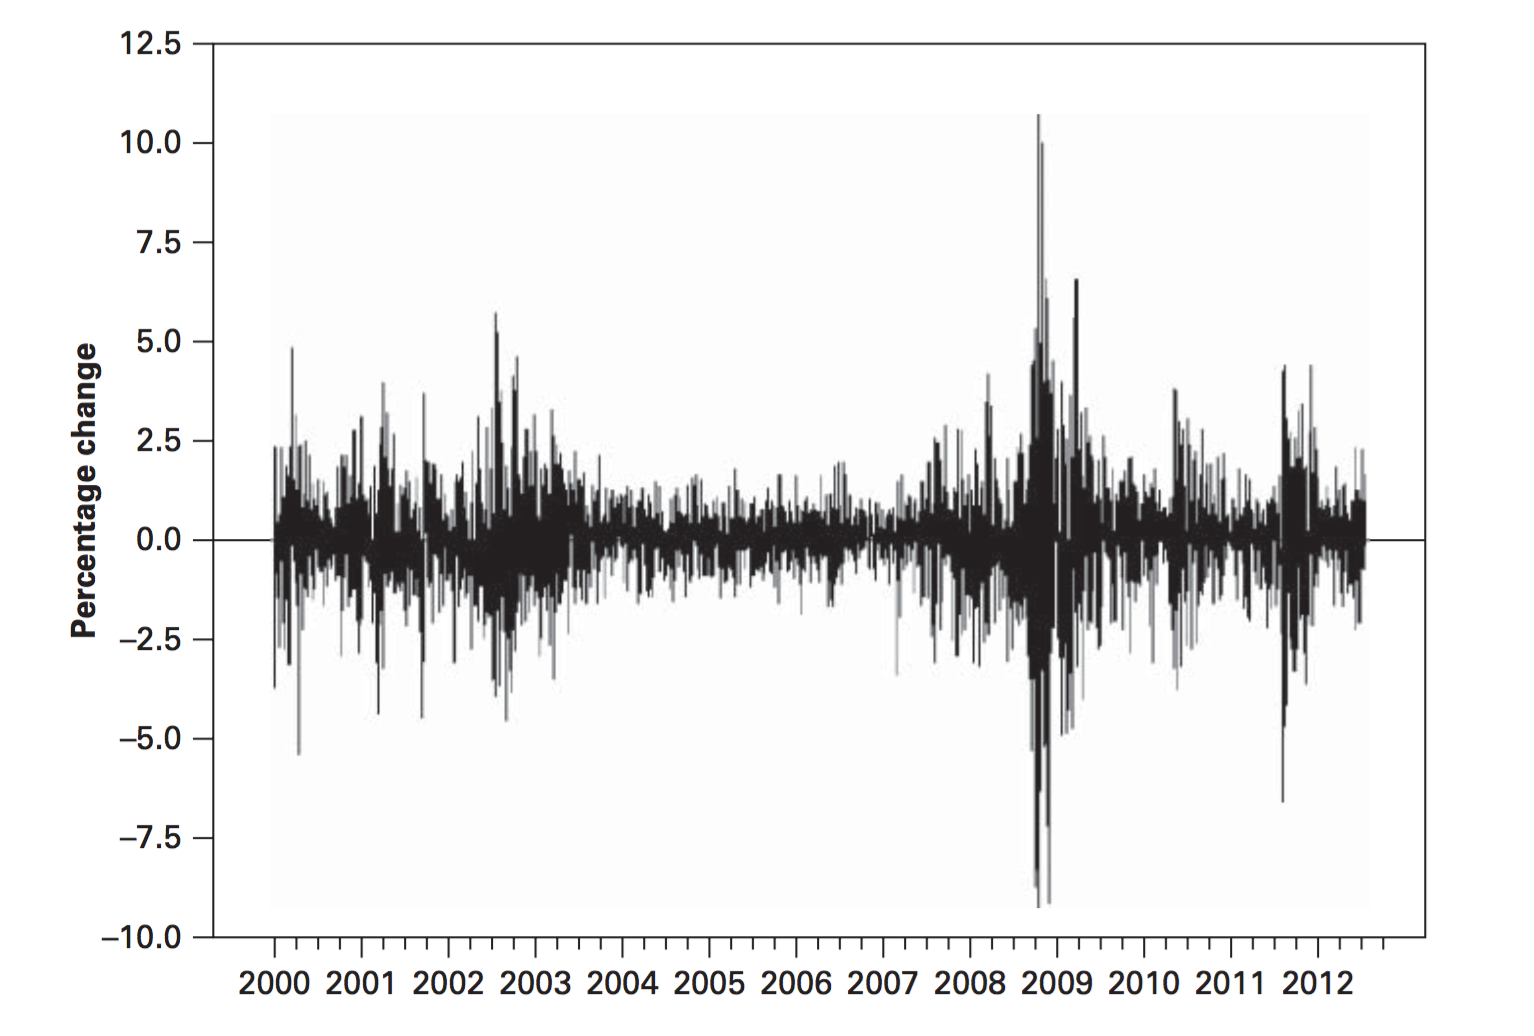
\includegraphics[width=0.7\textwidth]{img/nyse_us100.png}
\caption{\label{fig:orga9bc61e}
Percentage Change in the NYSE U.S.100 stock price index}
\end{figure}
\end{enumerate}
\end{frame}

\begin{frame}[label={sec:org620a743}]{Characteristics of volatility (2)}
\begin{enumerate}
\item Volatility evolves over time in a continuous manner. That is,
volatility jumps are rare.
\begin{figure}[htbp]
\centering
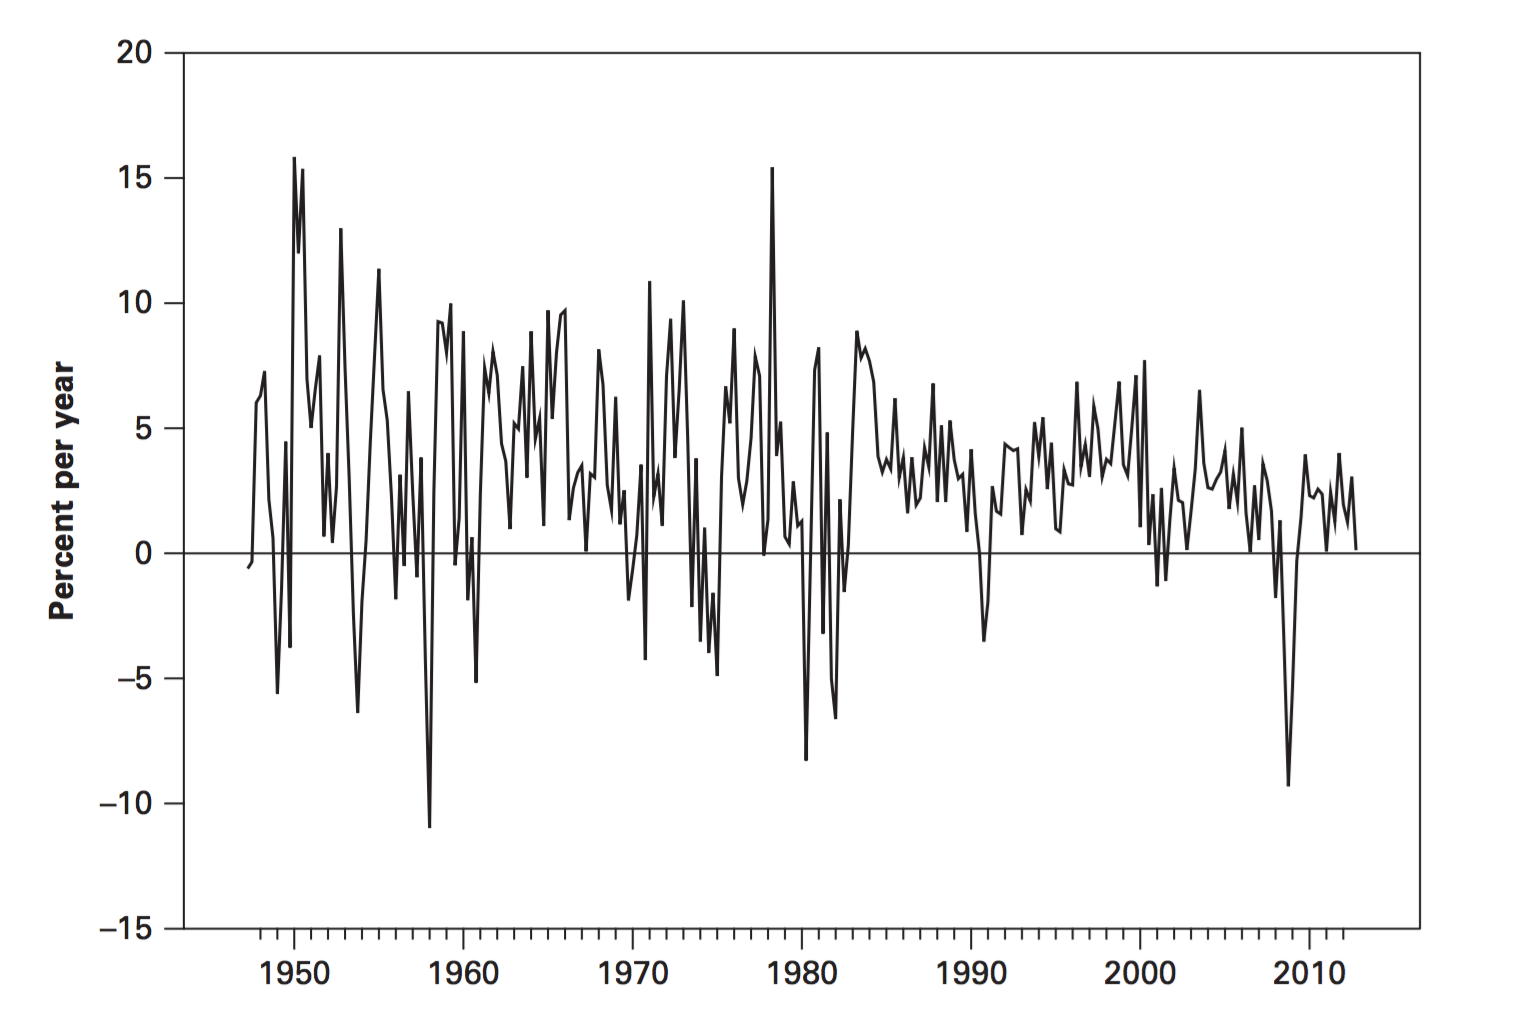
\includegraphics[width=0.7\textwidth]{img/readgdp.png}
\caption{\label{fig:org8d696d1}
Annualized Growth Rate of Real GDP}
\end{figure}
\end{enumerate}
\end{frame}

\begin{frame}[label={sec:orgf0fc011}]{Characteristics of volatility (3)}
\begin{enumerate}
\item Volatility does not diverge to infinity. That is, volatility varies
within some fixed range. Statistically speaking, this means that
volatility is often stationary.
\end{enumerate}

\vspace{0.5cm}

\begin{enumerate}
\item Volatility seems to react differently to a big price increase or a
big price drop, referred to as the leverage effect.
\end{enumerate}
\end{frame}

\section{The Structure of a Volatility Model}
\label{sec:orgbef7e6a}

\begin{frame}[label={sec:org71730ad}]{The basic idea of building a volatility model}
Consider the log return series \{\(r_t\)\}. The basic idea of a volatility
model is 
\begin{itemize}
\item \{\(r_t\)\} may appear to be either serially uncorrelated or
serially correlated with a minor order.
\item However, \{\(r_t\)\} is a dependent series and the dependence arises
from its conditional variance.
\end{itemize}

\begin{figure}[htbp]
\centering
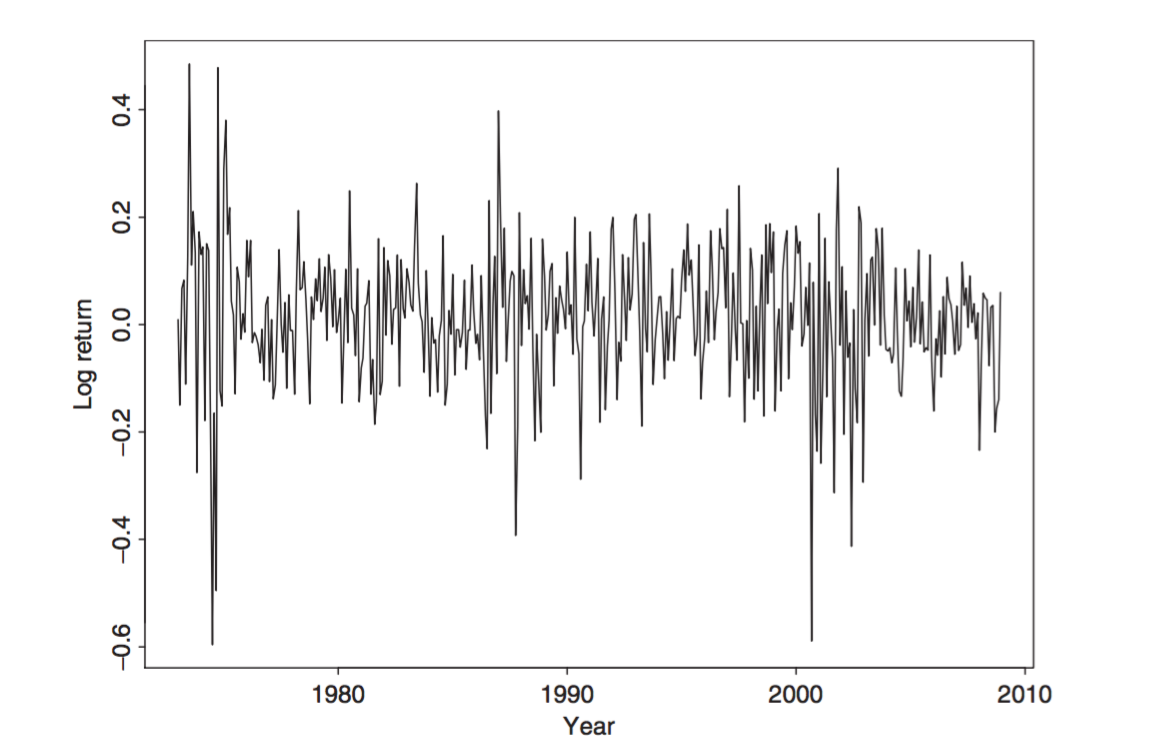
\includegraphics[width=0.7\textwidth,height=0.4\textheight]{img/intel.png}
\caption{\label{fig:org16a0235}
Time plot of monthly log returns of Intel stock from January 1973 to December 2008}
\end{figure}
\end{frame}

\begin{frame}[label={sec:org43ae204}]{The sample ACF of \{\(r_t\)\} and \{\(r^2_t\)\}}
\begin{figure}[htbp]
\centering
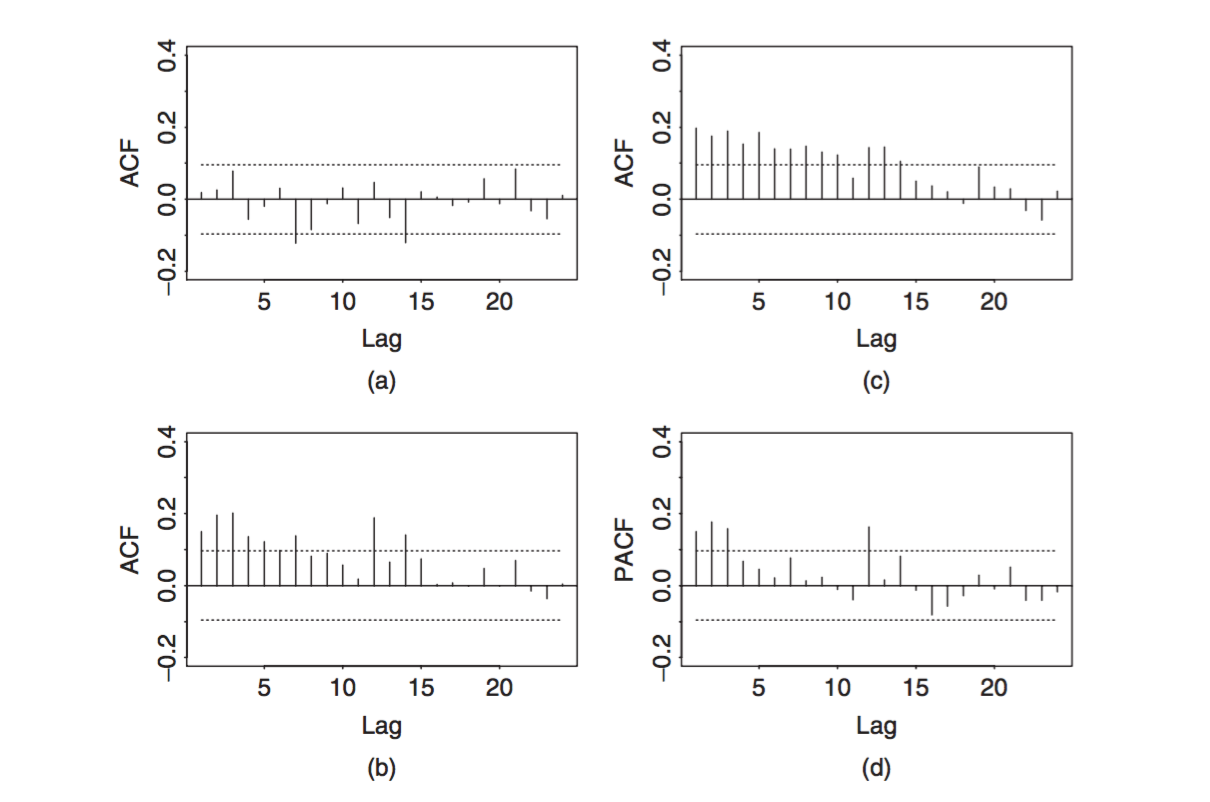
\includegraphics[width=0.9\textwidth,height=0.5\textheight]{img/acf_intel.png}
\caption{\label{fig:org6c18f6d}
Sample ACF and PACF of various functions of monthly log stock returns of Intel Corporation from January 1973 to December 2008: (a) ACF of the log returns, (b) ACF of the squared log returns, (c) ACF of the absolute log returns, and (d) PACF of the squared log returns.}
\end{figure}
\end{frame}

\begin{frame}[label={sec:orgab1f730}]{Decompose \(r_t\) into the mean and variance equations}
To capture the dependence in a time series through its second moment
but not the mean, we model the mean process and the variance process
separately. 

For a return series \{\(r_t\)\}, we can model it as
\begin{equation}
\label{eq:mean-plus-var}
r_t = \mu_t + a_t
\end{equation}
where \(\mu_t\) represents the conditional mean and \(a_t\) is
modeled to capture the conditional variance.
\end{frame}

\begin{frame}[label={sec:orgeabf2f0}]{The mean equation}
\begin{align}
&\mu_t = E(r_t \mid F_{t-1}) = \sum_{i=1}^p \phi_i y_{t-i} - \sum_{i=1}^q \theta_i a_{t-i} \label{eq:mean-equation} \\
&y_t = r_t - \phi_0 - \sum_{i=1}^k \beta_i x_{it} \nonumber
\end{align}
\(F_{t-1}\) is the information set at time \(t-1\). 

\vspace{0.5cm}

If you combine these two equations, and let \(\mu_t = r_t - a_t\), you
will find that it is just an ARMA\((p, q)\) model with additional
regressors \(x_{it}\).
\end{frame}

\begin{frame}[label={sec:orgcec7b98}]{The variance equation}
Denote the conditional variance of \(r_t\) with \(\sigma^2_t\).
\begin{equation*}
\begin{split}
\sigma^2_t = \var(r_t \mid F_{t-1}) &= E\left( (r_t - E(r_t | F_{t-1}))^2 | F_{t-1} \right) \\
&= E\left( (r_t - \mu_t)^2 \mid F_{t-1} \right) \\
&= \var(a_t \mid F_{t-1})
\end{split}
\end{equation*}
\end{frame}

\begin{frame}[label={sec:org8d503cf}]{The variance equation (cont'd)}
\begin{itemize}
\item If we assume that \(E(a_t \mid F_{t-1}) = 0\), we can see that
\(\sigma^2_t = E(a^2_t \mid F_{t-1})\). 

\vspace{0.3cm}

This result motivates us to use
the series of \{\(a^2_t\)\} to model the conditional variance
\(\sigma^2_t\).

\item The simplest model is a linear model, like the following
\[ \sigma^2_t = \alpha_0 + \alpha_1 a^2_{t-1} + \cdots + \alpha_m a^2_{t-m} \]

\item Let \(a^2_t = \sigma^2_t + \nu_t\) where \(\nu_t\) is a white noise
series. The above equation turns into an AR\((m)\) model for \{\(a^2_t\)\}
as follows
\[a^2_t = \alpha_0 + \alpha_1 a^2_{t-1} + \cdots + \alpha_m
  a^2_{t-m} + \nu_t \]
This equation represents the essential idea of an ARCH model with just
a little modification.
\end{itemize}
\end{frame}

\begin{frame}[label={sec:org2ce6672}]{The procedure of building a volatility model}
Building a volatility model for an asset return series consists of
four steps:

\begin{enumerate}
\item Specify a mean equation by testing for serial dependence in the
data and, if necessary, building an econometric model (e.g., an
ARMA model) for the return series to remove any linear dependence.

\item Use the squared residuals of the mean equation to test for ARCH
effects.

\item Specify a volatility model if ARCH effects are statistically
significant, and perform a joint estimation of the mean and
volatility equations.

\item Check the fitted model carefully and refine it if necessary.
\end{enumerate}
\end{frame}

\begin{frame}[label={sec:orgae61183}]{Testing for the presence of ARCH effect}
\begin{block}{The Ljung-Box test for the series of \(a^2_t\)}
Upon obtaining the residuals from the estimation
of an adequate mean equation, we can use the squared residuals
\{\(\hat{a}_t^2\)\} to test the existence of autocorrelation. 
\begin{itemize}
\item The Ljung-Box test is used to test the null hypothesis
\(H_0: \rho_1 = \cdots = \rho_m = 0\).
\item The \(Q(m)\) statistic is
calculated and compared with the critical value from \(\chi^2(m)\)
distribution at the desired significance level.
\item The rejection of the
null hypothesis implies that there is autoregressive conditional
heteroskedastic (ARCH) effect.
\end{itemize}
\end{block}
\end{frame}

\begin{frame}[label={sec:org384b386}]{The LM test}
\begin{block}{An auxiliary regression}
We estimate a AR\((m)\) model regarding \{\(\hat{a}^2_t\)\}, that is,
\[ \hat{a}^2_t = \alpha_0 + \alpha_1 \hat{a}_{t-1}^2 + \cdots +
\alpha_m \hat{a}^2_{t-m} + e_t \]
\end{block}

\begin{block}{The LM test}
With this model, we test the joint hypothesis
\[H_0: \alpha_1 = \cdots = \alpha_m = 0 \]
\begin{itemize}
\item The LM statistic is \(NR^2\) where \(N\) is the sample size of this
regression and \(R^2\) is the coefficient of the determination of this
regression.
\item Given the null hypothesis is true, this statistic follows
a \(\chi^2(m)\) distribution.
\end{itemize}
\end{block}
\end{frame}

\begin{frame}[label={sec:org051a076}]{The LM test (cont'd)}
Alternatively, we can use F statistic to test the joint
hypothesis. 
\begin{itemize}
\item Let \(SSR_0 = \sum_{t=m+1}^{T} (\hat{a}^2_{t} -
  \bar{\omega})^2\), where \(\bar{\omega} = (1/T) \sum_{t=1}^T
  \hat{a}^2_t\).
\item Let \(SSR_1 = \sum_{t=m+1}^T \hat{e}^2_t\) where \(\hat{e}_t\) is the
residuals from the regression.
\item The F statistic is
\[F = \frac{(SSR_0 - SSR_1)/m}{SSR_1/(T-2m-1)} \sim F(m, T-2m-1)\]
\item Rejecting the null hypothesis motivates us to model the possible
ARCH effect.
\end{itemize}
\end{frame}

\begin{frame}[label={sec:orgc0a598a}]{An example}
Go back to Figure \ref{fig:org6c18f6d}. Since the return series is
already stationary, we directly test the squared return series to
check the ARCH effect. 

\begin{itemize}
\item In the LM test of the ARCH effect, \(F = 53.62\) and the p value is
close to zero.
\item The Ljung–Box statistics of the \(a^2_t\) series also
shows strong ARCH effects with \(Q(12) = 89.85\), the p value of which is
close to zero.
\item Therefore, we can confirm that the return series of
Intel stock has an ARCH effect, and next we need to model such an
effect.
\end{itemize}
\end{frame}
\end{document}